\section{Background}

\begin{figure}
  \booltrue{commstr}
  \booltrue{commstl}
  \booltrue{commsbr}
  \booltrue{commsbl}
  \centering
  \documentclass[tikz]{standalone}
\usepackage{etoolbox} % for toggles

\newbool{commstr}
\newbool{commstl}
\newbool{commsbr}
\newbool{commsbl}

\booltrue{commstr}
\booltrue{commstl}
\booltrue{commsbr}
\booltrue{commsbl}

\begin{document}
\tikzstyle{proc} = [circle, draw=black, fill=lightgray]

\begin{tikzpicture}[]
  \matrix[row sep=0.75cm, column sep=1.5cm] {
    \node (A3) [proc] {}; &  \node (B3) [proc] {}; &  \node (C3) [proc] {}; \\
    \node (A2) [proc] {}; &  \node (B2) [proc] {}; &  \node (C2) [proc] {}; \\
    \node (A1) [proc] {}; &  \node (B1) [proc] {}; &  \node (C1) [proc] {}; \\
  };
 
  % Vertical dashed continuity lines
  \path[->]
    (A1) edge[thick, dashed] (A2) 
    (B1) edge[thick, dashed] (B2)
    (C1) edge[thick, dashed] (C2)
    (A2) edge[thick, dashed] (A3) 
    (B2) edge[thick, dashed] (B3)
    (C2) edge[thick, dashed] (C3)
  ;
 
  % Bottom level --> arrows
  \ifbool{commsbr}{
    \path[->]
      (A1) edge[thick] (B2)
      (B1) edge[thick] (C2)
    ;
  }{}
  % Bottom level <-- arrows
  \ifbool{commsbl}{
    \path[->]
      (B1) edge[thick] (A2)
      (C1) edge[thick] (B2)
    ;
  }{}
  % Top level --> arrows
  \ifbool{commstr}{
    \path[->]
      (A2) edge[thick] (B3)
      (B2) edge[thick] (C3)
    ;
  }{}
  % Top level <-- arrows
  \ifbool{commstl}{
    \path[->]
      (B2) edge[thick] (A3)
      (C2) edge[thick] (B3)
    ;
  }{}
  \end{tikzpicture}
\end{document}

  \caption{Conventional Communications Pattern}
  \label{fig:convcomms}
\end{figure}

\begin{figure}
  \centering
  \documentclass[tikz]{standalone}

\begin{document}
  \tikzset{>=latex} % Change default arrowhead to filled triangle
  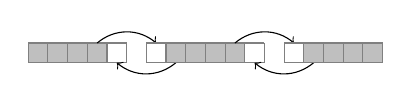
\begin{tikzpicture}[scale=0.25]
    \fill[lightgray] (0,0) rectangle (4,1);
    \draw[gray, step=1] (0,0) grid (5,1);
    
    \draw[->] (3.5,1) to [bend left=40] (6.5,1);
    \draw[->] (7.5,0) to [bend left=40] (4.5,0);

    \fill[lightgray] (7,0) rectangle (11,1);
    \draw[gray, step=1] (6,0) grid (12,1);
    
    \draw[->] (10.5,1) to [bend left=40] (13.5,1);
    \draw[->] (14.5,0) to [bend left=40] (11.5,0);

    \fill[lightgray] (14,0) rectangle (18,1);
    \draw[gray, step=1] (13,0) grid (18,1);

  \end{tikzpicture}
\end{document}

  \caption{Conventional 1D Boundary Exchange}
  \label{fig:exch1d}
\end{figure}

\begin{figure}
  \centering
  \documentclass[tikz]{standalone}

\begin{document}
  \tikzset{>=latex} % Change default arrowhead to filled triangle
  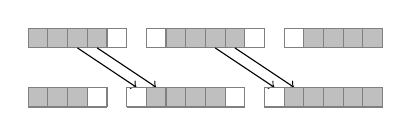
\begin{tikzpicture}[scale=0.25]

    % Timestep 1
    \fill[lightgray] (0,3) rectangle (4,4);
    \draw[gray, step=1] (0,3) grid (5,4);
    
    \fill[lightgray] (7,3) rectangle (11,4);
    \draw[gray, step=1] (6,3) grid (12,4);
    
    \fill[lightgray] (14,3) rectangle (18,4);
    \draw[gray, step=1] (13,3) grid (18,4);
   
   \draw[->](3.5,3) to (6.5,1);
   \draw[->](2.5,3) to (5.5,1);

   \draw[->](10.5,3) to (13.5,1);
   \draw[->](9.5,3) to (12.5,1);

    % Timestep 2
    \fill[lightgray] (0,0) rectangle (3,1);
    \draw[gray, step=1] (0,0) grid (4,1);
    
    \fill[lightgray] (6,0) rectangle (10,1);
    \draw[gray, step=1] (5,0) grid (11,1);
    
    \fill[lightgray] (13,0) rectangle (18,1);
    \draw[gray, step=1] (12,0) grid (18,1);


  \end{tikzpicture}
\end{document}

  \caption{Cascade 1D Boundary Exchange}
  \label{fig:trans1d}
\end{figure}

\begin{figure}
  \centering
  \documentclass[tikz]{standalone}
\usetikzlibrary{fit} % for node bounding boxes

\begin{document}
  \tikzstyle{sq} = [minimum height=0.8cm, minimum width=0.8cm]
  \tikzstyle{pe} = [rectangle, sq, draw=black]
  \tikzset{>=latex} % Change default arrowhead to filled triangle
  
  % \pelem[label]
  \def\pelem[#1] {
    \node (#1) [pe] {PE}; 
  }

  % \blank[label]
  \def\blank[#1] {
    \node (#1) [sq] {}; 
  }

  % \cgroup[from_node, to_node]
  \def\cgroup[#1, #2] {
    \node(group-#1-#2)[fit=(#1)(#2), thick, red, dashed, rounded corners, draw]{};
  }

  % \hlink[from_label, to_label]
  \def\hlink[#1, #2]{
    \draw[thick, ->] (#1.15) -- (#2.165);
    \draw[thick, <-] (#1.345) -- (#2.195);
  }

  % \vlink[from_label, to_label]
  \def\vlink[#1, #2]{
    \draw[thick, <-] (#1.285) -- (#2.75);
    \draw[thick, ->] (#1.255) -- (#2.105);
  }

  \begin{tikzpicture}[]
    \matrix[row sep=.5cm, column sep=.5cm] {
      \pelem[A0] & \pelem[B0] & \node(C0)[sq]{$\ldots$}; & \pelem[D0] & \pelem[E0] \\ 
      \pelem[A1] & \pelem[B1] & \blank[C1] & \blank[D1] & \pelem[E1] \\ 
      \node(A2)[sq]{$\vdots$}; & \blank[B2] & \node[sq](C2){$\ddots$}; & \blank[D2] & \node[sq](E2){$\vdots$}; \\ 
      \pelem[A3] & \blank[B3] & \blank[C3] & \pelem[D3] & \blank[E3] \\ 
      \pelem[A4] & \pelem[B4] & \node[sq](C4){$\ldots$}; & \blank[D4] & \pelem[E4] \\ 
    };

    % Center Control Group
    \cgroup[B1, D3]
    \node[red, below=0.4cm] at (group-B1-D3) {\textbf{CG1}};
   
    % Principal Compass Directions
    \cgroup[B0, D0]
    \node[red, above=0.6cm] at (group-B0-D0) {Control Group 2 \textbf{(CG2)}};
    \cgroup[B4, D4]
    \node[red, below=0.6cm] at (group-B4-D4) {\textbf{CG6}};
    \cgroup[A1, A3]
    \node[red, left=0.6cm] at (group-A1-A3) {\textbf{CG4}};
    \cgroup[E1, E3]
    \node[red, right=0.6cm] at (group-E1-E3) {\textbf{CG8}};

    % Corners
    \cgroup[A0, A0]
    \node[red, above left=0.6cm] at (group-A0-A0) {\textbf{CG3}};
    \cgroup[A4, A4]
    \node[red, below left=0.6cm] at (group-A4-A4) {\textbf{CG5}};
    \cgroup[E4, E4]
    \node[red, below right=0.6cm] at (group-E4-E4) {\textbf{CG7}};
    \cgroup[E0, E0]
    \node[red, above right=0.6cm] at (group-E0-E0) {\textbf{CG9}};
   
    % Horizontal Linkage
    \hlink[A0, B0] \hlink[B0, C0] \hlink[C0, D0] \hlink[D0, E0]
    \hlink[A1, B1] \hlink[B1, C1]                \hlink[D1, E1]
    % ...   
    \hlink[A3, B3]                \hlink[C3, D3] \hlink[D3, E3]
    \hlink[A4, B4] \hlink[B4, C4]                 \hlink[D4, E4]

    % Vertical Linkage
    \vlink[A0, A1] \vlink[B0, B1]                \vlink[D0, D1] \vlink[E0, E1]
    \vlink[A1, A2] \vlink[B1, B2]                               \vlink[E1, E2]
    \vlink[A2, A3]                               \vlink[D2, D3]               
    \vlink[A3, A4] \vlink[B3, B4]                \vlink[D3, D4] \vlink[E3, E4]
  \end{tikzpicture}
\end{document}

  \caption{Systolic Computational-Memory Array (SCMA)}
  \label{fig:scma}
\end{figure}
